\documentclass[11pt]{article}

\usepackage[a4paper,margin=1in]{geometry}
\usepackage{amsmath,amssymb}
\usepackage{graphicx}
\usepackage{booktabs}
\usepackage{float}
\usepackage{xcolor}
\usepackage{tikz}
\usetikzlibrary{arrows.meta,positioning}
\usepackage{hyperref}

\graphicspath{{../results/}}
\hypersetup{colorlinks=true, linkcolor=blue!50!black, urlcolor=blue!50!black, citecolor=blue!50!black}

\title{Nonparametric estimation of a density and its distribution function:\\
a Parzen Window study, and a neural network that improves on it}
\author{parzen-cdf project work}
\date{\today}

\newcommand{\Fhat}{\widehat{F}}
\newcommand{\fhat}{\widehat{f}}
\newcommand{\shat}{\hat{\sigma}}
\newcommand{\takeaway}[1]{\medskip\noindent\fcolorbox{black!30}{black!4}{\parbox{0.97\linewidth}{\textbf{Takeaway.} #1}}\medskip}

\begin{document}
\maketitle

\begin{abstract}
\noindent Given a finite sample and no assumption on the distribution it comes from, we
estimate the probability density function (pdf) and the cumulative distribution function
(CDF), in two stages. First, a \textbf{Parzen Window} estimator \cite{parzen1962} turns the
sample into a smooth estimate of the density, whose integral is the CDF estimate; with the
logistic window used here, that integral has a closed form. Second, a small feed-forward
neural network is trained to reproduce the CDF estimate at the sample points, in the spirit
of Parzen Neural Networks \cite{trentin2018}, and the density is read off as the derivative
of the network.

All experiments use synthetic data, so every estimate can be scored against a reference
curve of known precision. The study proceeds in small steps: it first calibrates the single
free parameter of the Parzen Window (the window size) with a systematic stress test, and
distills the outcome into a zero-cost rule of thumb that reaches the statistical accuracy
floor with as few as 500 samples. It then shows the main result: trained on
\emph{leave-one-out} Parzen targets computed with a deliberately sharp window, a
deliberately small network produces a density estimate 2 to 5 times more accurate than the
very Parzen Window it was trained from.
\end{abstract}

\tableofcontents

\section{Introduction}

\subsection{The task and the pipeline}

We are given $n$ real numbers $x_1, \dots, x_n$, drawn independently from an unknown
distribution, and nothing else. We want two functions of $x$:

\begin{itemize}
  \item the \textbf{density} (pdf) $f(x)$, describing where the data concentrates. It is
        never negative and the total area under it is 1;
  \item the \textbf{CDF} $F(x)$: the probability of observing a value smaller than or equal
        to $x$. It is the integral of the density, and it grows from 0 to 1.
\end{itemize}

No parametric form is assumed: the estimate must come from the sample alone. The pipeline
studied in this report does it in four moves (Figure~\ref{fig:pipeline}): a Parzen Window
estimator produces a first estimate of the density, and its integral gives the CDF estimate;
a small neural network is trained to reproduce that CDF estimate, using as training set
\emph{only} the sample points and the estimated values there; the network's derivative gives
back a density; a final inexpensive correction (\emph{rectification}: replace the network
output by its running maximum and rescale it to $[0,1]$) guarantees that the final CDF never
decreases and that the final density has total area exactly 1.

\begin{figure}[H]
\centering
\resizebox{\linewidth}{!}{%
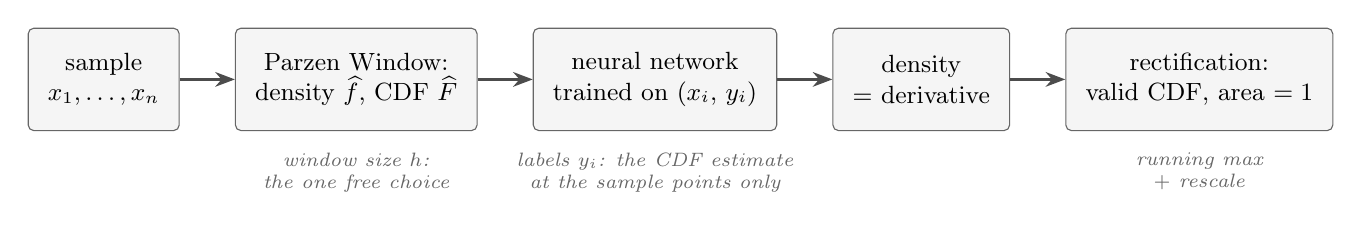
\begin{tikzpicture}[
  node distance=4mm and 7mm,
  box/.style={draw=black!60, rounded corners=2pt, fill=black!4, align=center,
              minimum height=13mm, inner sep=2.5mm, font=\small},
  lab/.style={font=\scriptsize\itshape, text=black!60, align=center},
  arr/.style={-{Stealth[length=2.5mm]}, thick, black!70}
]
\node[box] (s) {sample\\ $x_1,\dots,x_n$};
\node[box, right=of s] (pw) {Parzen Window:\\ density $\fhat$, CDF $\Fhat$};
\node[box, right=of pw] (net) {neural network\\ trained on $(x_i,\, y_i)$};
\node[box, right=of net] (der) {density\\ $=$ derivative};
\node[box, right=of der] (rect) {rectification:\\ valid CDF, area $=1$};
\draw[arr] (s) -- (pw);
\draw[arr] (pw) -- (net);
\draw[arr] (net) -- (der);
\draw[arr] (der) -- (rect);
\node[lab, below=1.5mm of pw] {window size $h$:\\ the one free choice};
\node[lab, below=1.5mm of net] {labels $y_i$: the CDF estimate\\ at the sample points only};
\node[lab, below=1.5mm of rect] {running max\\ $+$ rescale};
\end{tikzpicture}}%
\caption{The pipeline. Everything downstream depends on one free choice, the window size.}
\label{fig:pipeline}
\end{figure}

\subsection{How every estimate is scored}
\label{sec:scoring}

Two error measures are used throughout, one per estimated function.

\paragraph{CDF gap (KS).} Draw the estimated CDF and the reference CDF on the same axes; the
KS gap is the \textbf{largest vertical distance} between the two curves. It is a number
between 0 and 1; smaller is better.

\paragraph{Density error (ISE).} For densities we use the integrated squared error: the area
under the squared difference between estimated and reference density. Smaller is better.

Both measures compare a single estimator: the density estimate and the CDF estimate are the
same object (one is the integral of the other, with the same window size $h$). The two
scores, however, need not be minimized by exactly the same $h$, and Section~\ref{sec:gauss}
measures this.

\paragraph{Two fixed reference rows.} Every table in this report carries the same two
references, so that ``good'' has a concrete meaning:
\begin{itemize}
  \item the \textbf{empirical CDF}: the staircase that jumps by $1/n$ at every sample point.
        It is the estimate one gets for free, with no smoothing at all; any method worth
        using should beat it;
  \item the \textbf{statistical floor}: with $n$ independent samples, the expected KS gap of
        the empirical CDF is $\approx 0.87/\sqrt{n}$ (from the asymptotic law of the
        Kolmogorov statistic). No estimator can do systematically much better at a given
        $n$: it is the price of having observed only $n$ points. At $n = 500$, $1000$ and
        $2000$ the floor is $0.039$, $0.027$ and $0.019$ respectively.
\end{itemize}

\takeaway{An estimator is doing its job when its KS gap sits near the floor $0.87/\sqrt n$.
Once there, further accuracy can only come from more samples, not from a better method.}

\section{The Parzen Window estimator}

\subsection{Definition}

The Parzen Window estimate of the density at a point $x$ is
\begin{equation}
  \fhat(x) \;=\; \frac{1}{n} \sum_{i=1}^{n} \frac{1}{h}\,
  \varphi\!\left(\frac{x - x_i}{h}\right),
  \label{eq:pw}
\end{equation}
where the \emph{window function} $\varphi$ is any fixed function that is never negative and
has total area 1, and $h > 0$ is the \textbf{window size}
\cite{parzen1962,duda2001}. In words: place one bump of shape $\varphi$, width proportional
to $h$ and area $1/n$, on top of every sample, and add them up. Because each bump has area
$1/n$, the total area is automatically 1, so Eq.~\eqref{eq:pw} is a proper density for any
sample and any $h$.

Different window shapes are admissible under the same two conditions. Figure~\ref{fig:kernels}
shows the five shapes implemented in this project, all drawn at $h = 1$: they enclose the
same area but have different spreads (standard deviations from $0.41$ to $1.81$). This
matters when comparing window sizes across shapes: the effective amount of smoothing at a
given $h$ is proportional to the shape's spread, so a value of $h$ tuned for one shape does
not transfer to another unless it is rescaled by the ratio of the spreads.

\begin{figure}[H]
\centering
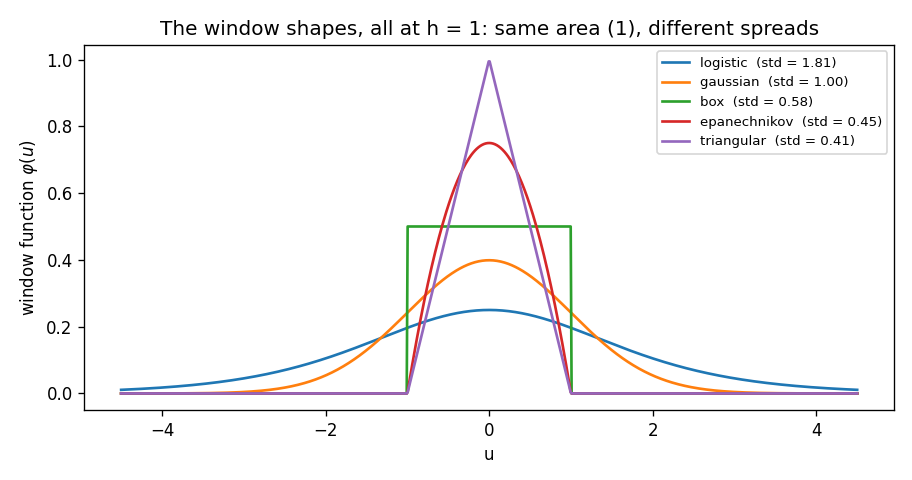
\includegraphics[width=0.75\linewidth]{report2_kernels.png}
\caption{Admissible window shapes, all with area 1, drawn at $h = 1$. Their spreads differ,
so the same $h$ produces different amounts of smoothing depending on the shape.}
\label{fig:kernels}
\end{figure}

\subsection{The logistic window and the CDF in closed form}

Throughout this study $\varphi$ is the \textbf{logistic} window,
$\varphi(u) = \sigma(u)\,(1-\sigma(u))$ with $\sigma(u) = 1/(1+e^{-u})$. Its integral is the
logistic sigmoid itself, so the CDF estimate (the integral of Eq.~\eqref{eq:pw}) has a
closed form:
\begin{equation}
  \Fhat(x) \;=\; \frac{1}{n} \sum_{i=1}^{n}
  \sigma\!\left(\frac{x - x_i}{h}\right).
  \label{eq:pwcdf}
\end{equation}
$\Fhat$ is smooth, strictly increasing, valued in $(0,1)$, and its exact derivative is
Eq.~\eqref{eq:pw}. This makes it a natural regression target for a network built from
sigmoids, which is the reason for the choice.

The implementation is verified rather than trusted, with three checks. As $h \to 0$,
Eq.~\eqref{eq:pwcdf} must reproduce the empirical CDF exactly, and it does (the measured
difference is $0$). For every window shape, the density must integrate to 1 and match the
numerical derivative of the CDF, and it does. With the gaussian window, Eq.~\eqref{eq:pw}
must agree with an independent implementation (\texttt{scipy.stats.gaussian\_kde}) at equal
$h$, and it does, with a maximum difference of $4 \cdot 10^{-16}$: machine precision.

\subsection{The window must shrink as the sample grows}
\label{sec:schedule}

For the estimate to converge to the underlying density as $n$ grows, the window size cannot
stay fixed: the classical conditions require the window to shrink (so that the estimate can
localize) but not too fast (so that each neighborhood still contains many samples)
\cite{duda2001}. A standard deterministic way to satisfy them is the schedule
\begin{equation}
  h_n \;=\; \frac{h_1}{\sqrt{n}},
  \label{eq:schedule}
\end{equation}
which leaves a single number to choose, the initial size $h_1$, once
\cite{duda2001}. Figure~\ref{fig:schedule} contrasts a window held constant with the
schedule, on a three-mode test density: the constant window's error freezes near $0.1$
regardless of $n$, while the scheduled window tracks the statistical floor.

\begin{figure}[H]
\centering
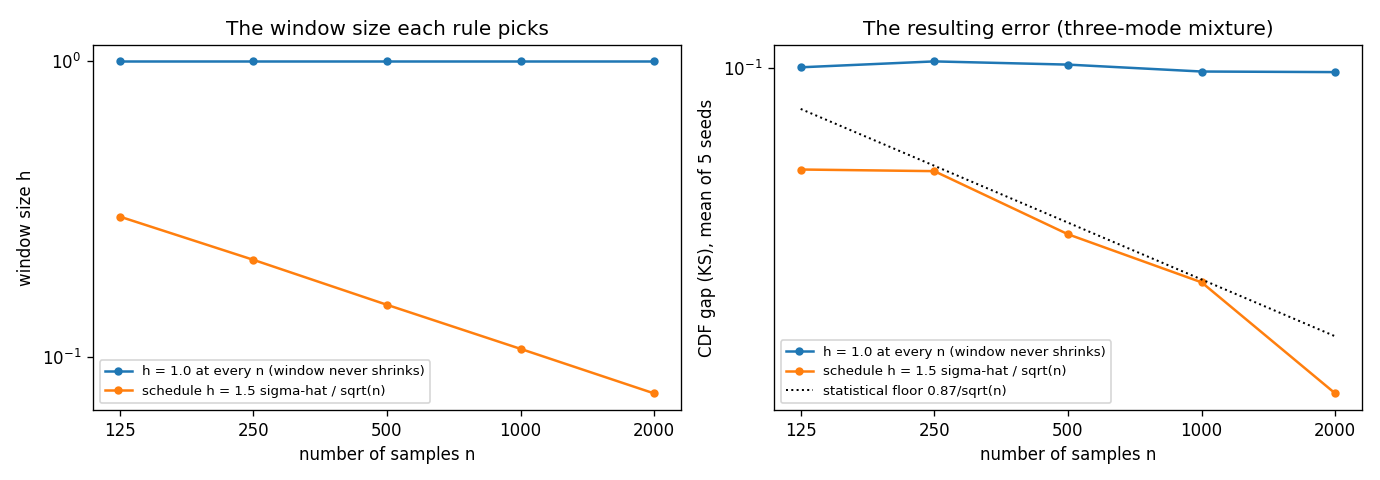
\includegraphics[width=\linewidth]{report2_schedule.png}
\caption{A window held constant against the schedule of Eq.~\eqref{eq:schedule}, on the
three-mode mixture of Section~\ref{sec:mixtures}. Left: the window size each rule picks as
$n$ grows. Right: the resulting CDF gap; the dotted line is the statistical floor.}
\label{fig:schedule}
\end{figure}

\subsection{The synthetic data and the reference curves}
\label{sec:data}

The test distributions are \textbf{mixtures of gaussians}: weighted sums of normal
components with assorted means, widths and weights. They are convenient for exactly one
reason: every quantity needed to score an estimate is computable to machine precision.
Precisely, and since nothing here should be taken for granted:

\begin{itemize}
  \item the reference \textbf{density} is a weighted sum of gaussian densities, which are
        elementary functions: it is evaluated in closed form;
  \item the reference \textbf{CDF} is a weighted sum of gaussian CDFs. The gaussian CDF has
        no closed form in terms of elementary functions, but it is
        $\Phi(z) = \tfrac12(1 + \operatorname{erf}(z/\sqrt2))$, and the error function
        $\operatorname{erf}$ is a standard special function that numerical libraries
        evaluate with a relative error of about $10^{-16}$. The gaps measured in this study
        are of order $10^{-2}$ to $10^{-3}$: thirteen orders of magnitude larger than the
        uncertainty of the reference. For every purpose of this report, the reference
        curves are exact;
  \item \textbf{sampling} from a mixture is exact and requires no CDF inversion: first draw
        which component generated the point (a categorical draw with the mixture weights),
        then draw from that gaussian component with a standard exact generator (the
        ziggurat method; such generators never touch the CDF). As an empirical check, a
        goodness-of-fit test of samples against the reference CDF, repeated over 40
        independent samples of size 1000, rejected at the 5\% level twice: exactly the
        expected false-alarm rate of a correct sampler.
\end{itemize}

Unless stated otherwise, every number in this report is a mean over repeated independent
samples (the exact counts are stated per experiment), the evaluation grid spans the mixture
support with 2001 points, and the sample budgets are $n = 500$ (baseline), $1000$ and
$2000$.

\section{Phase A: calibrating the window size}

The schedule of Eq.~\eqref{eq:schedule} reduces window-size selection to one number, $h_1$.
Phase A measures how much $h_1$ matters, extracts a rule of thumb for it, and tests the rule
on a battery of randomly generated mixtures against stronger (and costlier) selectors.

\subsection{Step 1: the single gaussian}
\label{sec:gauss}

The first test distribution is the standard normal $N(0,1)$. Table~\ref{tab:gauss-start}
starts from the most naive possible choice, $h_1 = 1.0$, with no tuning at all.

\begin{table}[H]
\centering
\begin{tabular}{lcccc}
\toprule
$n$ & $h = 1/\sqrt{n}$ & KS & empirical CDF & floor \\
\midrule
500  & 0.045 & \textbf{0.029} & 0.037 & 0.039 \\
1000 & 0.032 & \textbf{0.026} & 0.030 & 0.027 \\
2000 & 0.022 & \textbf{0.017} & 0.019 & 0.019 \\
\bottomrule
\end{tabular}
\caption{$N(0,1)$, schedule with the untuned start $h_1 = 1$ (mean over 10 samples): at the
floor and better than the empirical CDF at every budget.}
\label{tab:gauss-start}
\end{table}

Next, $h_1$ is \textbf{stress-tested}: 100 values spanning $[0.05, 30]$, at every budget
(Figure~\ref{fig:gaussstress}). Three observations:

\begin{enumerate}
  \item the KS optimum is broad and scale-linked: $h_1^* \approx 3.5$ to $4.3$, which is
        about $3.5$ times the sample standard deviation $\shat$, and any $h_1$ within a
        factor 3 to 4 of the optimum stays within 10\% of the best KS (the exact plateaus:
        $[2.3, 4.3]$ at $n = 500$, $[1.6, 5.2]$ at $1000$, $[1.4, 6.0]$ at $2000$);
  \item the optimum drifts slowly upward with $n$, by the predictable amount: the window
        size minimizing the CDF gap is known to scale as $n^{-1/3}$ \cite{azzalini1981},
        while the schedule imposes $n^{-1/2}$, so the best $h_1$ grows as $n^{1/6}$.
        Predicted drift from $n = 500$ to $2000$: $4^{1/6} = 1.26$; measured: $1.21$;
  \item \textbf{one estimator, two scores, two optima.} The density estimate and the CDF
        estimate share the same $h$, but the ISE of the density is minimized at a slightly
        larger $h_1$ than the KS of the CDF. The reason is mechanical: pointwise wiggle
        from a small window averages out when integrated into a CDF, so the KS tolerates
        under-smoothing well, while the density score sees the wiggle directly. When a
        single $h$ must serve both curves, erring slightly small protects the CDF and costs
        the density a little; the tables report both scores.
\end{enumerate}

\begin{figure}[H]
\centering
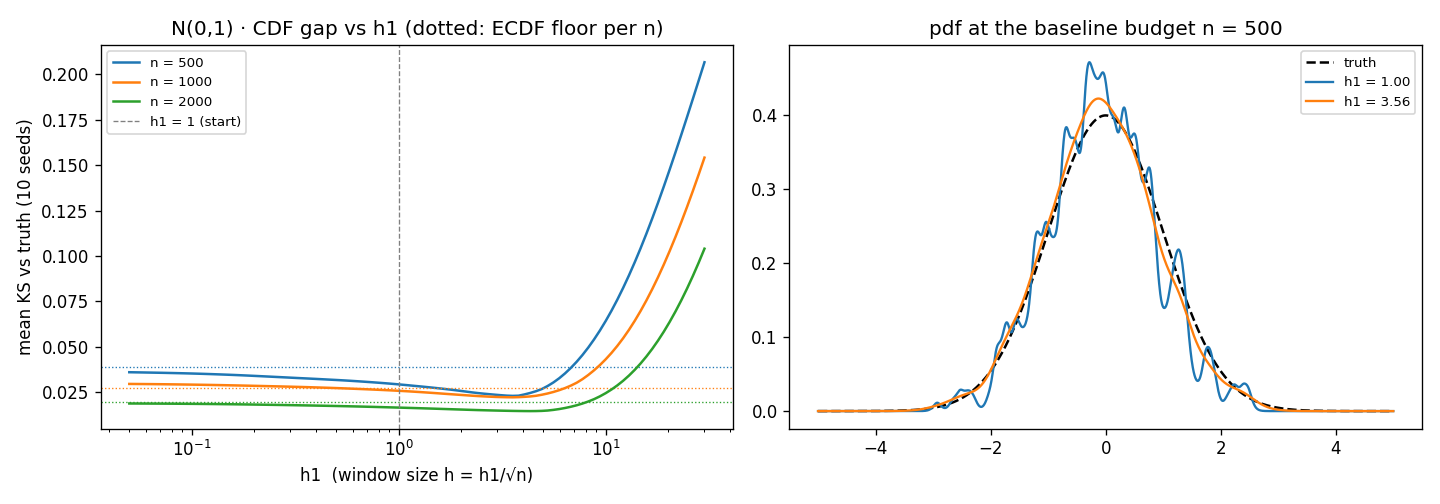
\includegraphics[width=\linewidth]{parzen2_gaussian_stress.png}
\caption{The $h_1$ stress test on $N(0,1)$ (100 values, mean over 10 samples). Left: KS
against $h_1$ per budget (dotted lines: the floors; vertical line: the untuned start).
Right: the density estimate at $n = 500$, with the untuned and the optimal $h_1$.}
\label{fig:gaussstress}
\end{figure}

\subsection{Step 2: multimodal mixtures, and the $h_1$ rule of thumb}
\label{sec:mixtures}

The same stress test is repeated on three multimodal mixtures: a symmetric bimodal (two
equal, well-separated modes), an asymmetric bimodal (unequal weights and widths, partial
overlap), and an asymmetric trimodal (three modes, one narrow), which serves as the running
example of the study.

\begin{table}[H]
\centering
\small
\begin{tabular}{llccccccc}
\toprule
distribution & $n$ & $h_1^*$ & KS$^*$ & KS at $h_1{=}1$ & empirical & floor & 10\% plateau & $h_1^*/\shat$ \\
\midrule
symmetric bimodal   & 500  & 2.8 & 0.035 & 0.039 & 0.044 & 0.039 & [0.9, 4.3] & 1.3 \\
                    & 1000 & 2.8 & 0.022 & 0.024 & 0.028 & 0.027 & [1.0, 4.6] & 1.3 \\
                    & 2000 & 3.6 & 0.014 & 0.015 & 0.017 & 0.019 & [0.7, 5.2] & 1.7 \\
asymmetric bimodal  & 500  & 3.3 & 0.027 & 0.031 & 0.037 & 0.039 & [1.6, 4.9] & 2.0 \\
                    & 1000 & 4.3 & 0.022 & 0.026 & 0.029 & 0.027 & [1.6, 6.4] & 2.6 \\
                    & 2000 & 3.1 & 0.014 & 0.015 & 0.017 & 0.019 & [0.6, 6.0] & 1.9 \\
asymmetric trimodal & 500  & 2.4 & 0.033 & 0.034 & 0.039 & 0.039 & [0.5, 4.3] & 1.1 \\
                    & 1000 & 2.8 & 0.025 & 0.026 & 0.029 & 0.027 & [0.6, 4.6] & 1.2 \\
                    & 2000 & 2.4 & 0.015 & 0.016 & 0.018 & 0.019 & [0.3, 4.6] & 1.1 \\
\bottomrule
\end{tabular}
\caption{The $h_1$ stress test on the multimodal ladder (100 values of $h_1$, mean over 10
samples). The ``10\% plateau'' is the range of $h_1$ whose KS stays within 10\% of the
optimum.}
\label{tab:mixtures}
\end{table}

\begin{figure}[H]
\centering
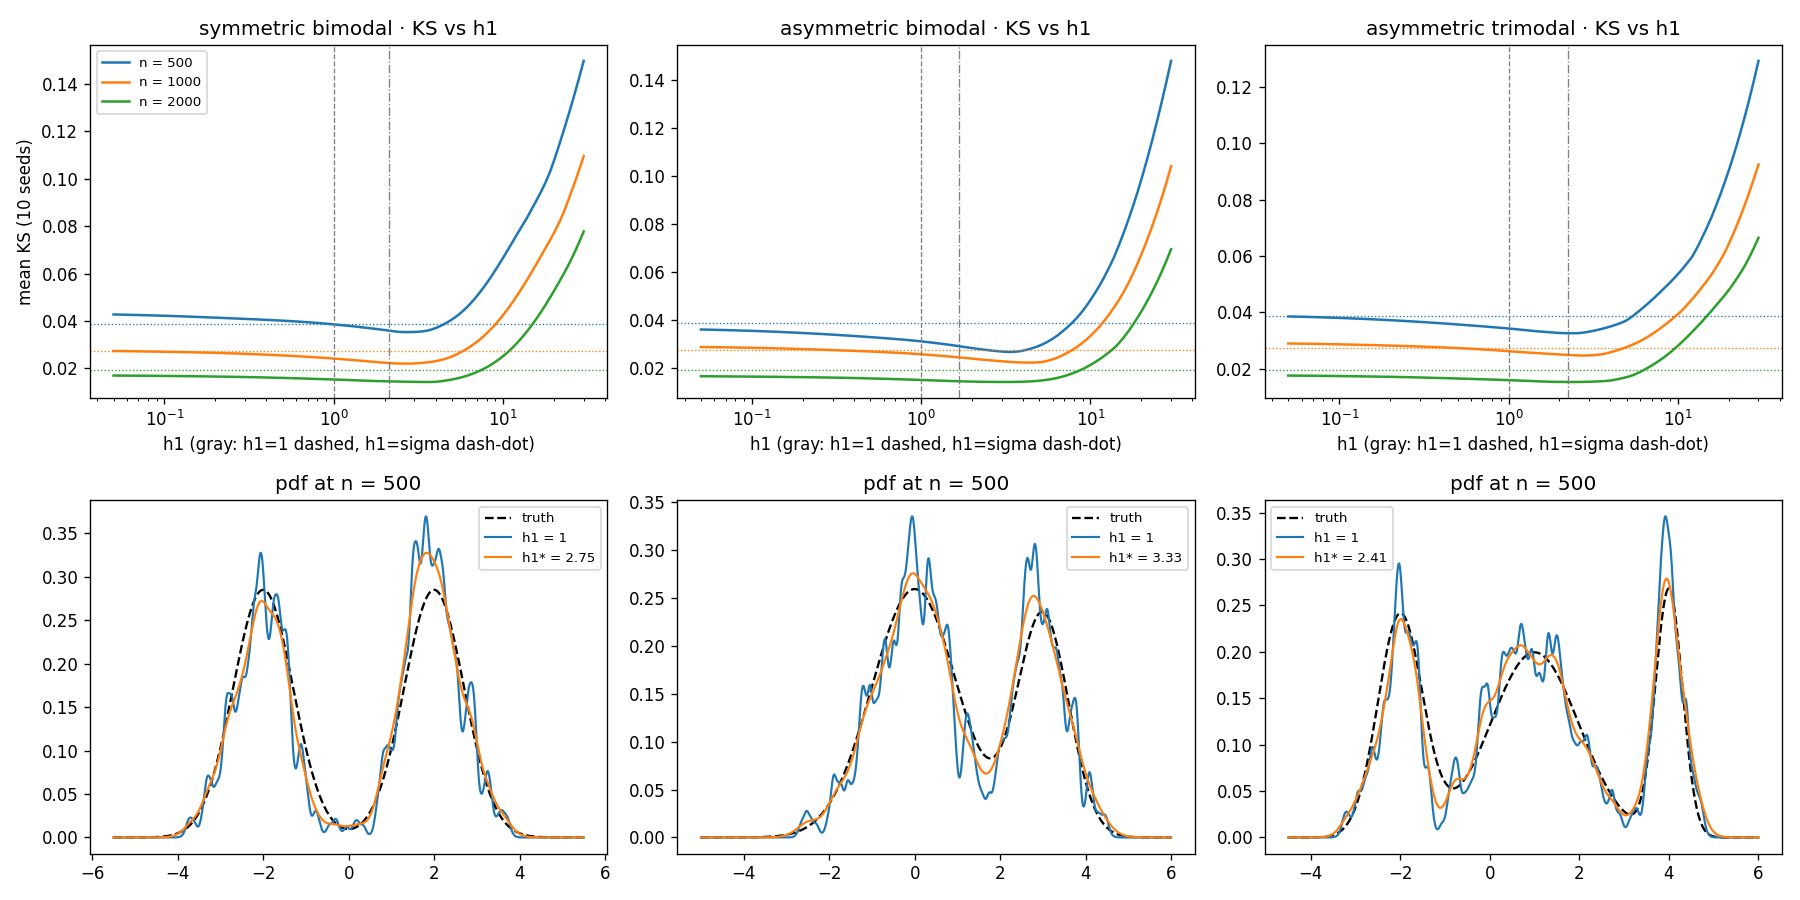
\includegraphics[width=\linewidth]{parzen2_mixtures_stress.png}
\caption{Top: KS against $h_1$ for the three mixtures (vertical lines: $h_1 = 1$ dashed,
$h_1 = \shat$ dash-dotted). Bottom: the density estimates at the baseline $n = 500$, with
the untuned and the optimal $h_1$. All three modes of the trimodal are resolved with 500
samples.}
\label{fig:mixstress}
\end{figure}

Two structural facts set up the rule of thumb. First, multimodality pulls the optimum down,
to $h_1^* \approx 1.1$ to $2.6$ times $\shat$ (against $3.5$ for the gaussian): the window
must resolve the narrowest feature of the density, not its overall spread. Second, the
error is \textbf{asymmetric} around the optimum: the KS curves are nearly flat to its left
and rise steeply to its right, so a rule of thumb should err on the small side. Combining
the two, and using the sample standard deviation as the natural scale (a practice with
precedent in Parzen-based classifiers \cite{specht1990}):

\begin{center}
\fcolorbox{black!40}{black!4}{\parbox{0.7\linewidth}{\centering
\textbf{$\sigma$-rule}\quad $h_1 = 1.5\,\shat$,\qquad i.e.\qquad
$h_n = \dfrac{1.5\,\shat}{\sqrt{n}}$}}
\end{center}

\noindent It is truth-free, costs one standard deviation to compute, and is scale-invariant:
the bare $h_1 = 1$ performs identically on these particular datasets only because they
happen to have $\shat \approx 1$ to $2$, and would fail on data measured in different units.

\subsection{Step 3: a battery of ten random mixtures}
\label{sec:batteryA}

The rule is then evaluated on ten randomly generated mixtures (3 to 6 gaussian components
each, means, widths and weights drawn at random once and then fixed), three independent
samples per mixture and budget. The $\sigma$-rule was frozen \emph{before} this battery was
run. Alongside it:

\begin{itemize}
  \item \textbf{LSCV} (least-squares cross-validation): a standard data-driven selector
        that scores each candidate window on the sample itself via a leave-one-out
        criterion and picks the best; its cost grows with $n^2$. Candidates: 40 values on a
        geometric grid from $0.01\,\shat$ to $0.5\,\shat$;
  \item the \textbf{oracle}: the fixed window that minimizes the \emph{measured} KS against
        the reference CDF, chosen separately for each sample set. It uses the reference
        curve, which no data-driven method can access: it is reported as an upper bound on
        what window selection could possibly achieve;
  \item the empirical CDF and the floor, as always.
\end{itemize}

\begin{table}[H]
\centering
\begin{tabular}{lccc}
\toprule
selector & $n=500$ & $n=1000$ & $n=2000$ \\
\midrule
start ($h_1 = 1$)                        & 0.031 & 0.025 & 0.016 \\
\textbf{$\sigma$-rule ($h_1 = 1.5\shat$)} & 0.031 & 0.025 & 0.015 \\
LSCV (cost $\sim n^2$)                   & 0.030 & 0.023 & 0.015 \\
\midrule
oracle fixed $h$ (uses the reference)    & 0.028 & 0.022 & 0.014 \\
empirical CDF                            & 0.036 & 0.028 & 0.018 \\
floor $0.87/\sqrt n$                     & 0.039 & 0.027 & 0.019 \\
\bottomrule
\end{tabular}
\caption{Mean KS over the battery (10 mixtures $\times$ 3 samples). The $\sigma$-rule
matches cross-validation at zero cost and stays within 10 to 15\% of the oracle.}
\label{tab:battery}
\end{table}

\begin{figure}[H]
\centering
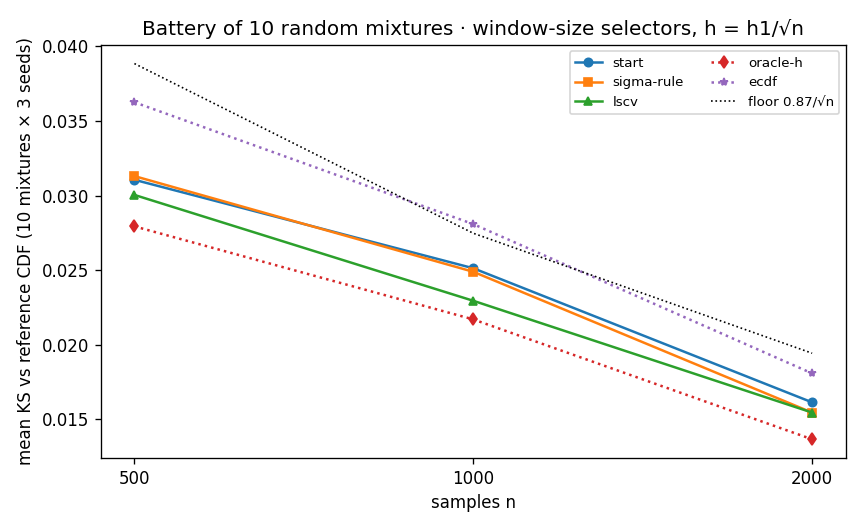
\includegraphics[width=0.7\linewidth]{parzen2_random_selectors.png}
\caption{The battery at a glance: all schedule-based selectors track the floor.}
\label{fig:batteryA}
\end{figure}

\begin{figure}[H]
\centering
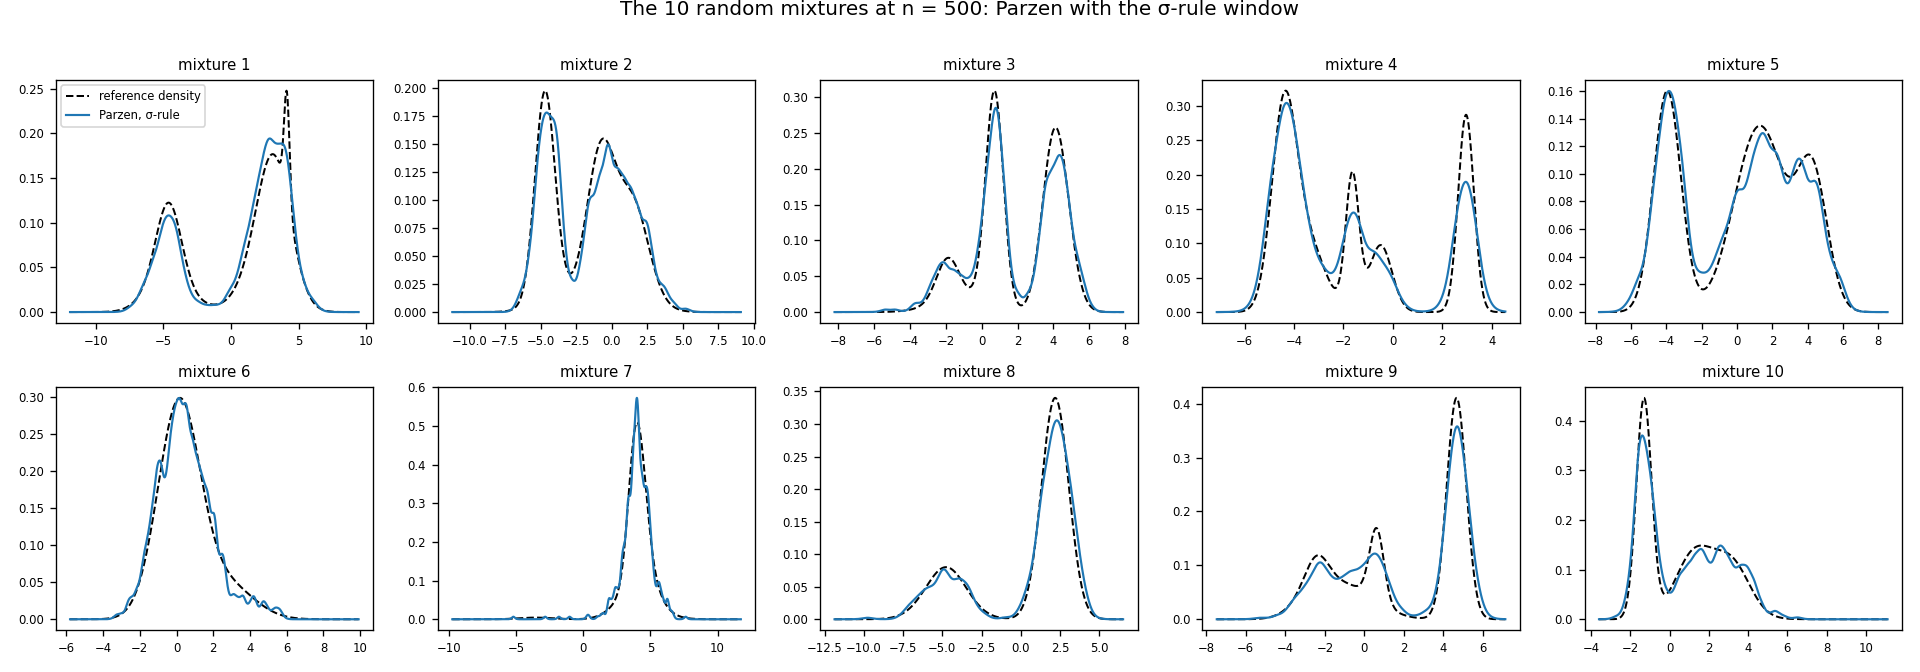
\includegraphics[width=\linewidth]{parzen2_random_gallery.png}
\caption{The ten mixtures of the battery at the baseline budget $n = 500$: reference density
(dashed) and the Parzen estimate with the $\sigma$-rule window.}
\label{fig:galleryA}
\end{figure}

\takeaway{With the window given by the $\sigma$-rule, the Parzen Window sits at the
statistical floor on every distribution tested, from $n = 500$ upward. Window selection
reduces to one robust, zero-cost rule of thumb; cross-validation buys 5 to 10\% more at
$n^2$ cost, and even a reference-using oracle only 10 to 15\%.}

\section{Phase B: a network that improves on its teacher}

\subsection{The idea}

A network trained to reproduce a good estimate can, at best, match it. The Parzen Neural
Network (PNN) construction \cite{trentin2018} escapes this ceiling with three coordinated
choices:

\begin{enumerate}
  \item the targets are computed with a \textbf{deliberately sharp window} (smaller than
        optimal). Such an estimate follows the underlying curve closely \emph{on average}
        but is very noisy (the thin curve in Figure~\ref{fig:pnn}, left);
  \item each target is computed \textbf{leave-one-out}: the label at $x_i$ uses every
        sample except $x_i$ itself. Otherwise every label would contain a spurious bump
        contributed by its own sample point, an offset that does not average away;
  \item the network is \textbf{deliberately small}. A small network cannot represent the
        noise even if it tries: fitting the labels forces it through the middle of them,
        keeping the trend and discarding the fluctuations. Capacity acts as the
        regularizer.
\end{enumerate}

Around the underlying curve, the leave-one-out labels fluctuate with mean zero; a smooth
function of limited flexibility fitted through zero-mean fluctuations lands closer to the
underlying curve than the labels themselves. This is the mechanism by which the student can
end up more accurate than its teacher, and it also delimits it: if the teacher is already
smooth (little noise), there is nothing to remove and no gain to expect.

\subsection{The recipe, on the CDF}
\label{sec:recipe}

Here the PNN construction is applied to the CDF rather than the density. The teacher is the
logistic Parzen CDF of Eq.~\eqref{eq:pwcdf} with a sharp window,
$h_n = 0.5\,\shat/\sqrt{n-1}$ ($\sqrt{n-1}$ because each leave-one-out estimate averages
$n-1$ windows).

The leave-one-out labels have a closed form, derived in two lines. The full estimate at a
sample point contains that point's own window, evaluated at distance zero:
\begin{equation}
  \Fhat(x_i) \;=\; \frac{1}{n}\sum_{j=1}^{n} \sigma\!\left(\frac{x_i - x_j}{h}\right)
  \;=\; \frac{1}{n}\Big(\underbrace{\sigma(0)}_{=\,1/2}
        \;+\; \sum_{j \neq i} \sigma\!\big(\tfrac{x_i - x_j}{h}\big)\Big).
\end{equation}
Solving for the sum over the other $n-1$ samples and averaging over them:
\begin{equation}
  y_i \;=\; \frac{1}{\,n-1\,}\sum_{j \neq i} \sigma\!\left(\frac{x_i - x_j}{h}\right)
      \;=\; \frac{n\,\Fhat(x_i) - \tfrac12}{\,n-1\,}.
  \label{eq:loo}
\end{equation}
So the label at $x_i$ is exactly the CDF estimate that the \emph{other} $n-1$ samples
produce at $x_i$: the sample being labeled never contributes to its own label.

A one-hidden-layer network with sigmoidal activations and a sigmoidal output is trained by
full-batch gradient descent (Adam, 6000 epochs) on the pairs $(x_i, y_i)$ \textbf{only}: no
extra evaluation points, no augmentation. The density is the derivative of the trained
network, and rectification guarantees a never-decreasing CDF whose density has area exactly
1. This guarantee is worth a remark: a network trained to output a \emph{density} directly
has no such cheap fix, because forcing a function to integrate to 1 requires evaluating an
integral \cite{trentin2018,magdon2002}; on the CDF route the same guarantee costs one
running maximum.

\subsection{Network size: small wins}

With a sharp teacher ($h_1 = 0.5\,\shat$, trimodal, $n = 1000$, 5 samples), the hidden
width was scanned:

\begin{table}[H]
\centering
\begin{tabular}{lcc}
\toprule
hidden width & net KS & net density ISE \\
\midrule
\textbf{8}  & 0.028 & \textbf{0.0021} \\
16          & 0.028 & 0.0022 \\
32          & 0.043 & 0.0133 \\
64          & 0.059 & 0.0179 \\
\midrule
the teacher itself & 0.028 & 0.0043 \\
\bottomrule
\end{tabular}
\caption{Width 8 halves the teacher's density error; widths 32 and 64 are \emph{worse than
the teacher}, because they have enough capacity to fit its noise.}
\label{tab:capacity}
\end{table}

The width is frozen at 8 for everything that follows.

\subsection{Net against teacher, across regimes}

Teacher sharpness and budget are then swept: five sharpness levels
$h_1 \in \{0.25, 0.5, 1.0, 1.5, 3.0\} \cdot \shat$, budgets 500 to 2000, five samples each
(Figure~\ref{fig:pnn}).

\begin{figure}[H]
\centering
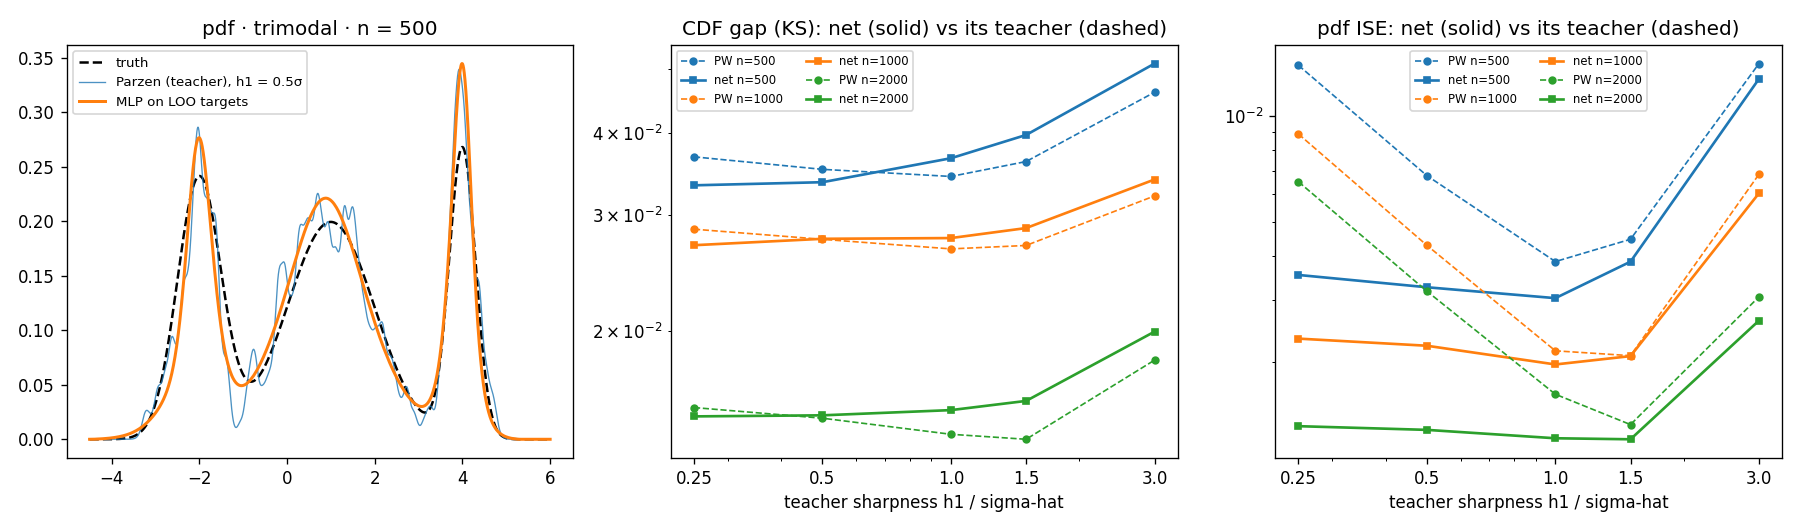
\includegraphics[width=\linewidth]{mlp2_pnn_cdf.png}
\caption{Left: the summary picture. The sharp Parzen teacher (thin line) is noisy; the
width-8 network trained on its leave-one-out labels (thick line) is smooth and close to the
reference. Middle and right: KS and density ISE of the network (solid) against its own
teacher (dashed) as the teacher's sharpness varies.}
\label{fig:pnn}
\end{figure}

\begin{itemize}
  \item On the \textbf{density}, the network beats the teacher it learned from by a factor
        2 to 5 when the teacher is sharp, fading to parity as the teacher approaches its
        own optimal smoothness (no noise left to remove);
  \item on the \textbf{CDF} the gain is small, as the mechanism predicts: integrating into
        a CDF is itself a smoothing operation, so the teacher's KS is nearly noise-free
        already. The noise reappears amplified under differentiation, which is exactly
        where the network's smoothness pays;
  \item the network is nearly \textbf{insensitive to the teacher's sharpness} (the flat
        solid curves in the right panel): once the teacher is sharp enough, the network
        extracts the same smooth estimate from it. The window-size selection problem,
        Phase A's central concern, nearly disappears from the network's side of the
        pipeline;
  \item at the baseline $n = 500$ the network also beats the best truth-free Parzen of
        Phase A ($\sigma$-rule) on both scores: KS $0.034$ vs $0.036$, density ISE
        $0.0033$ vs $0.0045$.
\end{itemize}

\subsection{Enforcing monotonicity: in the loss, or downstream}
\label{sec:mono}

A CDF must never decrease, and nothing in the training above enforces it. Several options
exist, and they were compared head-to-head under the frozen recipe (trimodal, 5 samples per
budget): \emph{raw} (nothing enforced, as a control); \emph{rectification} (the running-max
correction, applied after training); a \emph{soft penalty} added to the loss,
$\lambda \cdot \mathrm{mean}(\max(0, -\Fhat'))$ evaluated at 256 points spanning the
support, for $\lambda = 1, 10, 100$; and \emph{Sill} monotone-by-construction networks
(all weights kept positive through a reparameterization), which cannot decrease anywhere by
design \cite{sill1998}.

\begin{table}[H]
\centering
\small\setlength{\tabcolsep}{4pt}
\begin{tabular}{lccc@{\hskip 4mm}ccc@{\hskip 4mm}ccc@{\hskip 4mm}c}
\toprule
 & \multicolumn{3}{c}{$n=500$} & \multicolumn{3}{c}{$n=1000$} & \multicolumn{3}{c}{$n=2000$} & \\
\cmidrule(lr){2-4}\cmidrule(lr){5-7}\cmidrule(lr){8-10}
regime & KS & ISE & viol\,\% & KS & ISE & viol\,\% & KS & ISE & viol\,\% & mass \\
\midrule
raw                 & 0.033 & 0.0032 & 3.1 & 0.027 & 0.0022 & 1.7 & 0.014 & 0.0013 & 1.9 & 0.988 \\
rectified           & 0.035 & 0.0032 & 0   & 0.027 & 0.0022 & 0   & 0.015 & 0.0013 & 0   & \textbf{1.000} \\
penalty $\lambda=1$   & 0.033 & 0.0031 & 1.9 & 0.027 & 0.0021 & \textbf{0} & 0.015 & 0.0013 & 0.8 & 0.990 \\
penalty $\lambda=10$  & 0.034 & 0.0033 & 1.9 & 0.029 & 0.0027 & 0   & 0.015 & 0.0015 & 0.8 & 0.988 \\
penalty $\lambda=100$ & 0.039 & 0.0076 & 1.9 & 0.034 & 0.0051 & 0   & 0.020 & 0.0040 & 0.8 & 0.979 \\
Sill                & 0.034 & 0.0035 & \textbf{0} & 0.027 & \textbf{0.0021} & \textbf{0} & 0.015 & 0.0016 & \textbf{0} & 0.986 \\
\bottomrule
\end{tabular}
\caption{Monotonicity enforcement under the PNN-CDF recipe (trimodal, mean over 5 samples).
``viol'' is the fraction of grid steps where the delivered curve decreases (for
``rectified'' and ``Sill'' it is zero by construction); ``mass'' is the area of the
recovered density, averaged over the budgets (its variation across budgets is below
$0.003$).}
\label{tab:mono}
\end{table}

Three facts stand out. First, the raw violations are small but real (2 to 3\% of grid
steps). Second, a \emph{gentle} loss penalty ($\lambda = 1$) reduces or eliminates them at
no accuracy cost, while a strong one ($\lambda = 100$) fights the data term and doubles the
density error without fixing more. Third, and notably, the monotone-by-construction network
costs essentially nothing here: with a small network fitted to noisy leave-one-out targets,
Sill's constraint matches the unconstrained accuracy while guaranteeing zero violations
everywhere, not only on the evaluation grid. No in-training option, however, delivers a
density of area exactly 1: that guarantee only comes from the downstream rescaling, which
composes with any of them. The practical recipe is therefore either
\emph{rectification alone} (simplest) or \emph{Sill + rectification} (monotone everywhere,
area exactly 1).

\subsection{The battery}
\label{sec:batteryB}

Finally, the frozen recipe (width 8, teacher $h_1 = 0.5\,\shat$, leave-one-out labels,
rectification) is run on the same ten random mixtures as Phase A, three samples per mixture
and budget.

\begin{table}[H]
\centering
\small
\begin{tabular}{lcccccc}
\toprule
 & \multicolumn{3}{c}{CDF gap (KS)} & \multicolumn{3}{c}{density error (ISE)} \\
\cmidrule(lr){2-4}\cmidrule(lr){5-7}
estimator & $n{=}500$ & $n{=}1000$ & $n{=}2000$ & $n{=}500$ & $n{=}1000$ & $n{=}2000$ \\
\midrule
Parzen teacher ($0.5\,\shat$) & 0.030 & 0.027 & 0.021 & 0.0052 & 0.0042 & 0.0037 \\
\textbf{network (PNN-CDF)}    & \textbf{0.030} & 0.026 & 0.021 & \textbf{0.0027} & 0.0022 & 0.0015 \\
Parzen $\sigma$-rule          & 0.031 & 0.025 & 0.019 & 0.0033 & 0.0021 & 0.0014 \\
empirical CDF                 & 0.035 & 0.031 & 0.023 &        &        &        \\
floor                         & 0.039 & 0.027 & 0.019 &        &        &        \\
\bottomrule
\end{tabular}
\caption{Battery means (10 mixtures $\times$ 3 samples). Against the teacher it was trained
from, the network is better on the density in 27 of 30 mixture-budget cases (by $2\times$
on average) and better on the KS in 20 of 30.}
\label{tab:phaseB}
\end{table}

\begin{figure}[H]
\centering
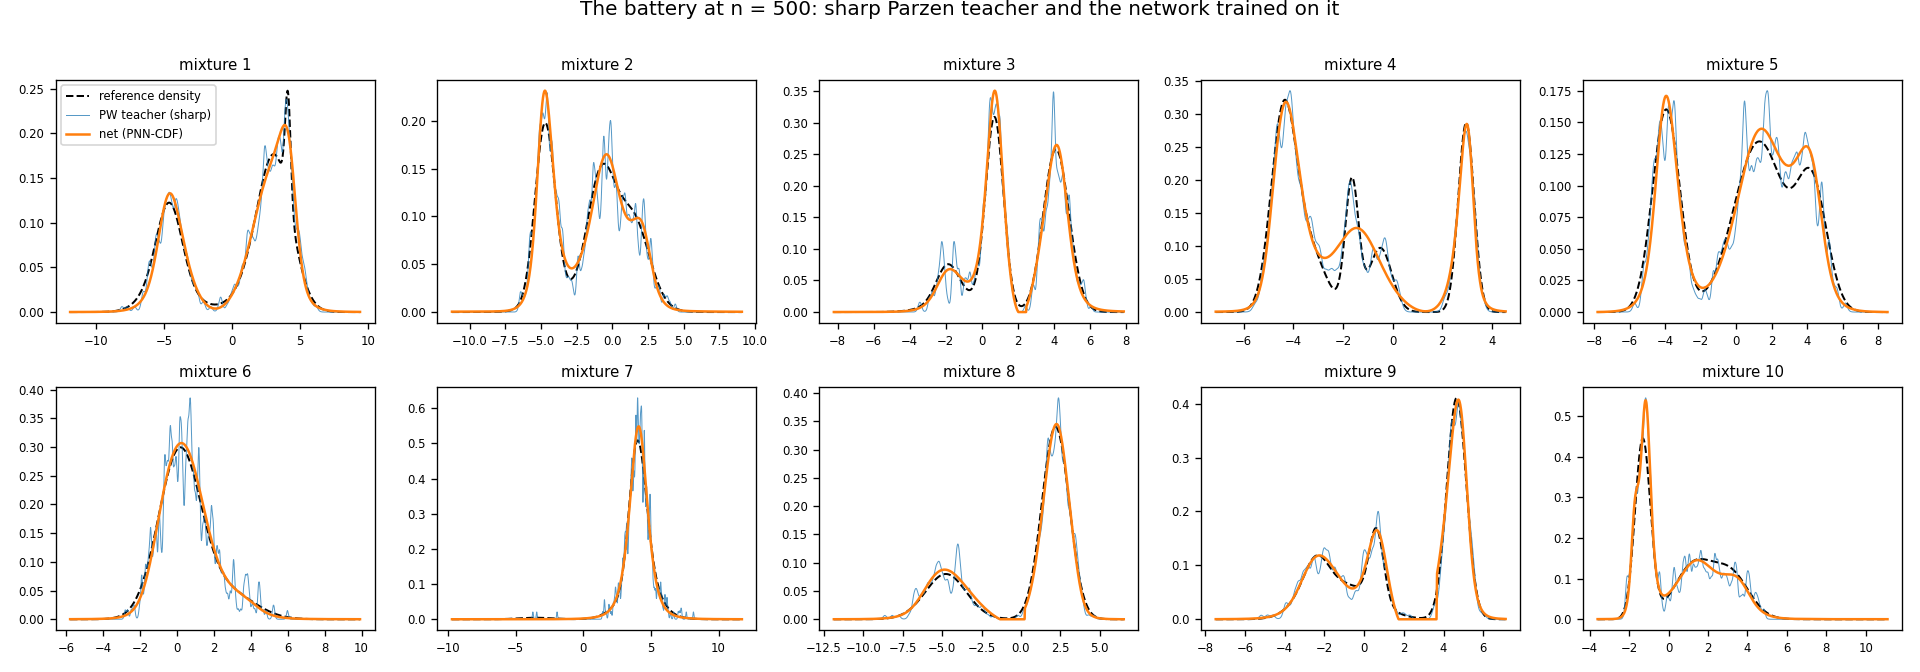
\includegraphics[width=\linewidth]{mlp2_battery_gallery.png}
\caption{The battery at $n = 500$: reference density (dashed), the sharp Parzen teacher
(thin), and the network trained on its leave-one-out labels (thick).}
\label{fig:galleryB}
\end{figure}

\begin{figure}[H]
\centering
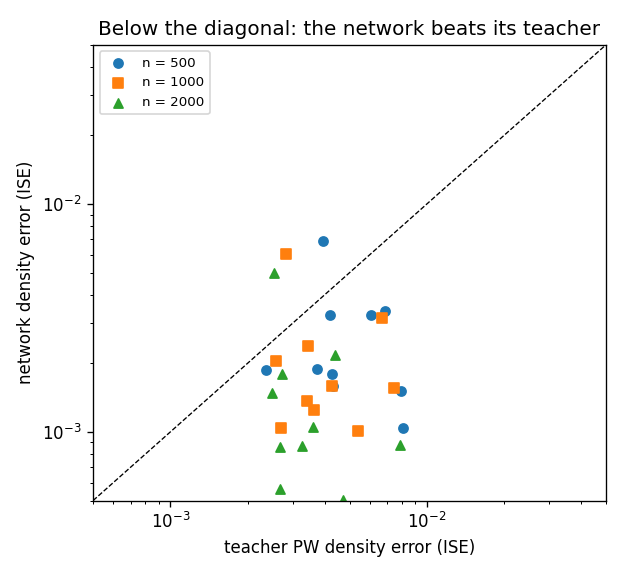
\includegraphics[width=0.55\linewidth]{mlp2_battery_scatter.png}
\caption{Density error of the network against that of its own teacher, one point per
mixture and budget. Points below the diagonal: the network is more accurate than the
estimator that produced its training labels.}
\label{fig:scatterB}
\end{figure}

\takeaway{Trained only at the sample points, on labels produced by a sharp leave-one-out
Parzen Window, a width-8 sigmoidal network yields a density estimate about twice as accurate
as that Parzen Window across the battery (27 of 30 cases; up to $5\times$ with sharper
teachers), and at $n = 500$ it also beats the best truth-free Parzen Window available. The
advantage is a small-sample advantage: by $n = 2000$ a well-sized Parzen Window ties on the
density. The CDF route additionally guarantees, at negligible cost, what a direct density
network cannot: a valid CDF and a density of total area 1.}

\section{Conclusions}

\begin{enumerate}
  \item \textbf{The Parzen Window, sized by the schedule $h_n = h_1/\sqrt n$ with the
        $\sigma$-rule $h_1 = 1.5\,\shat$, reaches the statistical accuracy floor with 500
        samples} on every distribution tested, from the single gaussian to random mixtures
        with up to six modes. The choice of $h_1$ is forgiving (a factor 3 to 4 of slack
        costs less than 10\%) and the rule is scale-invariant and free.
  \item \textbf{A small sigmoidal network trained on sharp leave-one-out Parzen targets
        improves on its own teacher}, by a factor 2 to 5 on the density where the teacher
        is noisy, and it is nearly insensitive to the teacher's window size. The gain
        concentrates on the density rather than the CDF, and at small samples rather than
        large: both facts follow from the mechanism (variance removal by limited capacity).
  \item \textbf{Monotonicity can be enforced in the loss or by construction at no accuracy
        cost in this regime}: a gentle penalty ($\lambda = 1$) removes most violations for
        free, and Sill networks remove all of them while matching the unconstrained
        accuracy. A density of area exactly 1, however, only comes from the downstream
        rescaling, which composes with either; strong penalties ($\lambda = 100$) hurt
        accuracy without fixing more.
\end{enumerate}

Open directions: per-case selection of the network width by cross-validated likelihood
\cite{trentin2018}; the multivariate extension, where the analogue of monotonicity (the
N-increasing property of joint CDFs) is the known technical obstacle.

\appendix

\section{Reproducibility}

All numbers and figures are produced by the scripts in \texttt{scripts/}, with fixed random
seeds:

\begin{itemize}
  \item Phase A: \texttt{parzen2\_gaussian.py}, \texttt{parzen2\_mixtures.py},
        \texttt{parzen2\_random.py};
  \item Phase B: \texttt{mlp2\_pnn\_cdf.py}, \texttt{mlp2\_monotonicity.py},
        \texttt{mlp2\_battery.py};
  \item Figures~\ref{fig:kernels} and~\ref{fig:schedule}: \texttt{report2\_figures.py};
        shared helpers: \texttt{study2\_common.py};
  \item verification of the estimator implementation and of the sampling:\\
        \texttt{temp\_analysis/verify\_formulation.py}.
\end{itemize}

\begin{thebibliography}{9}
\bibitem{parzen1962} E. Parzen, ``On estimation of a probability density function and
mode'', \emph{Annals of Mathematical Statistics} 33(3), 1962.
\bibitem{duda2001} R. O. Duda, P. E. Hart, D. G. Stork, \emph{Pattern Classification},
2nd ed., Wiley, 2001 (chapter 4: nonparametric techniques).
\bibitem{azzalini1981} A. Azzalini, ``A note on the estimation of a distribution function
and quantiles by a kernel method'', \emph{Biometrika} 68(1), 1981.
\bibitem{specht1990} D. F. Specht, ``Probabilistic neural networks'', \emph{Neural
Networks} 3(1), 1990.
\bibitem{trentin2018} E. Trentin, ``Parzen neural networks: fundamentals, properties, and
an application to forensic anthropology'', \emph{Neural Networks} 97, 2018.
\bibitem{magdon2002} M. Magdon-Ismail, A. Atiya, ``Density estimation and random variate
generation using multilayer networks'', \emph{IEEE Transactions on Neural Networks} 13(3),
2002.
\bibitem{sill1998} J. Sill, ``Monotonic networks'', \emph{Advances in Neural Information
Processing Systems} 10, 1998.
\end{thebibliography}

\end{document}
